%\cleardoublepage
%\newpage
%\thispagestyle{empty}
\mbox{}

\chapter{Análisis hiperespectral}
\label{ch:chapter2}

\section{Imágenes hiperespectrales}

Una imagen hiperespectral (o imagen de gran resolución espectral) es una imagen en la que cada punto (píxel) viene descrito por un conjunto (vector) de valores espectrales que se corresponden con la reflectancia de dicho píxel en diferentes longitudes de onda a estrechas bandas del espectro \cite{biblio:image_clasification}. Cada uno de esos vectores conforman lo que se denomina “firma espectral” \cite{biblio:hyper_analysis, biblio:Tesis_Carlos} del píxel en cuestión, y se obtienen gracias a los sensores hiperespectrales en diversos canales espectrales. El número de bandas que se utilizan suele variar desde las decenas hasta los varios centenares, y el conjunto no está limitado estrictamente al espectro visible sino que también abarca el infrarrojo y el ultravioleta. 

Se puede ver como un caso particular de las imágenes hiperespectrales a las imágenes RGB \cite{biblio:TFM_Pablo_VCA}, las más comunmente utilizadas en el día a día. Ellas están compuestas por tres bandas de color y cada una corresponde a una longitud de onda concreta: rojo, verde y azul, respectivamente. Para componer una imagen RGB a partir de una imagen hiperespectral, se pueden seleccionar esas tres longitudes de onda concretas o las más aproximadas que se encuentren.

Para el estudio de imágenes hiperespectrales se hace uso de la propiedad de reflectancia espectral \cite{biblio:TFG_Esquembri}, que es el porcentaje de energía reflejada sobre la energía incidente como una función de la longitud de onda. La reflectancia es característica de cada material porque varía en función de las distintas longitudes de onda para la mayoría de los materiales dado que la energía puede ser absorbida o reflejada en distintos grados. Por ello, el análisis de estas imágenes sirve también para identificar un material a partir de su firma espectral.

Una imagen hiperespectral puede ser representada como un cubo (denominado “hipercubo” o “cubo hiperespectral”) en el que los ejes X, denominado “líneas” (lines), e Y, denominado “muestras” (samples), se utilizan para mostrar la ubicación espacial de cada píxel de la imagen. El tercer eje Z, denominado “bandas” (bands), se utiliza para mostrar la reflectancia de cada píxel en cada uno de los canales espectrales que haya obtenido el sensor. En la Figura~\ref{fig:cubo hiperespectral} \cite{biblio:TFG_Esquembri} se muestra un ejemplo de cubo hiperespectral, en el que se pueden observar las diferentes bandas de longitudes de onda por separado.

\begin{figure}
  \centering
    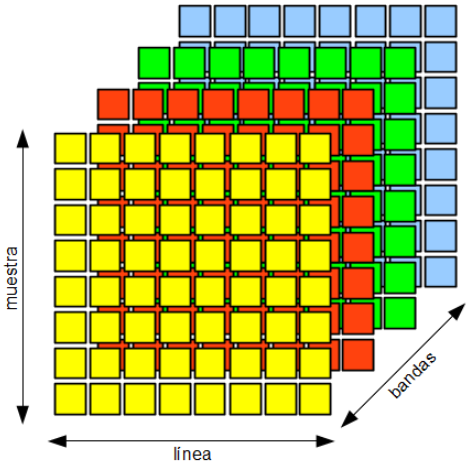
\includegraphics[width=0.5\textwidth]{Imagenes/CuboHiperespectral.png}
  \caption{Ejemplo de cubo hiperespectral.}
  \label{fig:cubo hiperespectral}
\end{figure}

Como se puede observar en la Figura~\ref{fig:pixeles puros y pixeles mezcla} \cite{biblio:TFM_Pablo_VCA}, existen dos tipos de píxeles en función de sus firmas espectrales. Si su firma espectral está constituida por un único tipo de material, el píxel se denomina píxel puro o endmember. Si, por el contrario, está constituida por varios materiales distintos a nivel de subpíxel, el píxel se denomina píxel mezcla. Estos últimos serán los que conformen la mayor parte de la imagen hiperespectral, ya que es muy habitual que cohabiten materiales diferentes en una misma porción de espacio, incluso a nivel microscópico. \cite{biblio:x}.

\begin{figure}
  \centering
    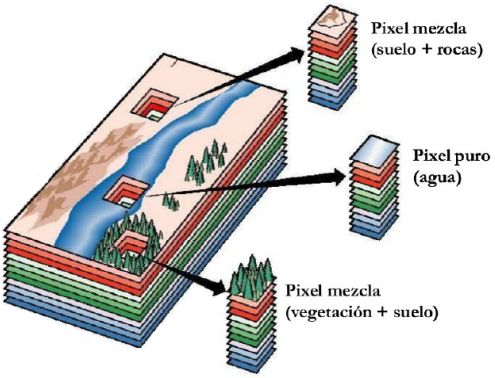
\includegraphics[width=0.6\textwidth]{Imagenes/PixelesPurosPixelesMezcla.png}
  \caption{Ejemplo de píxeles puros y píxeles mezcla.}
  \label{fig:pixeles puros y pixeles mezcla}
\end{figure}

Otro de los aspectos importantes a destacar de este tipo de imágenes es la resolución espectral \cite{biblio:TFM_Pablo_VCA}, que es la separación entre longitudes de onda (a menor separación, mayor resolución espectral) y viene determinada por la tecnología del sensor que se emplea. Cuanto mayor sea la resolución espectral, más información se obtendrá y se podrán esperar mejores resultados en el análisis de las imágenes. Sin embargo, es conveniente tener en cuenta que esta ventaja supone también un aumento considerable del coste computacional.

Las imágenes hiperespectrales surgieron a raíz de las imágenes multiespectrales \cite{landgrebe2003stm}. Este tipo de imágenes se diferencia de las anteriores en que la separación entre bandas es muy grande y la imagen dispone de un número muy pequeño de las mismas (de 4 a 20 aproximadamente). A pesar de basarse en los mismos conceptos, la información proporcionada por las imágenes multiespectrales es mucho más limitada y, por tanto, sus aplicaciones y su método de procesamiento son diferentes \cite{biblio:TFM_Pablo_VCA}.

\section{Sensores hiperespectrales}

El análisis de la Tierra nunca ha dejado de despertar interés o de ser objeto de estudio. Su observación remota se lleva realizando desde hace más de un centenar de años, tradicionalmente empleando cámaras instaladas en globos dirigibles o satélites. No fue hasta el inicio de los años 90 cuando comenzó a surgir la tecnología que serviría para desarrollar los sensores hiperespectrales.

Para obtener las imágenes hiperespectrales, los sensores se basan en la espectroscopia \cite{biblio:TFG_Esquembri}, que es el estudio de la luz emitida o reflejada por los materiales y su variación de energía con la longitud de onda. Esto se consigue empleando unos instrumentos llamados espectrómetros de imágenes, que son capaces de realizar mediciones espectrales de bandas muy próximas entre sí.

El concepto de imagen hiperespectral tuvo su origen en el Jet Propulsion Laboratory\footnote{https://www.jpl.nasa.gov}, una misión comercial de la NASA encargada del desarrollo de instrumentación para la adquisición de imágenes hiperespectrales, esto es, sensores de gran resolución espacial. Un ejemplo de esta instrumentación es el sensor Airborne Visible Infra-Red Imaging Spectrometer (AVIRIS)\footnote{https://aviris.jpl.nasa.gov}.

\subsection{Sensor AVIRIS}

AVIRIS es un sensor óptico creado en 1987 capaz de captar imágenes hiperespectrales de 224 canales espectrales (bandas) con longitudes de onda que varían entre 400 y 2500 nanómetros. Tiene la capacidad de obtener información con un ancho entre bandas (resolución espectral nominal) de 10 nanómetros. Está pensado para ser aerotransportado y analizar zonas del espectro visible e infrarrojo \cite{biblio:result_aviris,biblio:aviris_analysis}.

Este sensor ha realizado tomas de imágenes hiperespectrales en Europa, Estados Unidos, Canadá, Argentina y otras partes de América del Sur mediante el uso de cuatro plataformas de aviones: el jet ER-2, perteneciente al Jet Propulsion Laboratory de la NASA, que vuela a aproximadamente 20 kilómetros sobre el nivel del mar con una velocidad de unos 730 km/h; el turbopropulsor Twin Otter International, desarrollado por la compañía canadiense Havilland Canada, que vuela a 4 kilómetros sobre el nivel del suelo a una velocidad de 130 km/h; el Proteus de Scaled Composites; y el WB-57 de la NASA.

El objetivo principal del proyecto AVIRIS es identificar, medir y monitorizar los componentes de la superficie y la atmósfera terrestre basándose en la absorción molecular y las firmas de dispersión de partículas. Se trata de una investigación centrada principalmente en comprender los procesos relacionados con el medio ambiente y el cambio climático.

%En la Figura~\ref{fig:sensor aviris} se puede observar una imagen de este sensor.

%\begin{figure}
%  \centering
%    \includegraphics{}
%  \caption{Sensor AVIRIS}
%  \label{fig:sensor aviris}
%\end{figure}

\subsection{Sensor EO-1 Hyperion}

Este sensor fue lanzado con éxito en noviembre del año 2000 gracias al programa New Millenium\footnote{http://nmp.nasa.gov} de la NASA. Es capaz de obtener información con una resolución espacial de 30 metros y en 220 bandas espectrales, cubriendo un rango de longitudes de onda de entre 400 y 2500 nanómetros. Cada línea de datos en las imágenes hiperespectrales tomadas está constituida por 256 píxeles.

%En la Figura~\ref{fig:sensor eo-1 hyperion} se puede observar una imagen de este sensor.

%\begin{figure}
%  \centering
%    \includegraphics{}
%  \caption{Sensor EO-1 Hyperion}
%  \label{fig:sensor eo-1 hyperion}
%\end{figure}

\section{Bibliotecas espectrales}

Existen bibliotecas espectrales que facilitan el tratamiento y el análisis de imágenes hiperespectrales. Esto se debe a que contienen una elevada cantidad de datos de reflectancia espectral tanto de materiales naturales como desarrollados por el ser humano. A continuación se nombran algunas de ellas.

\subsection{Biblioteca espectral USGS}

Esta biblioteca fue desarrollada por el laboratorio de espectrometría United States Geological Survey (USGS)\footnote{https://www.usgs.gov}, en Colorado. Contiene información de en torno a 500 reflectancias espectrales, principalmente de minerales, sobre longitudes de onda que varían entre 0.2 y 3.0 micrómetros.

\subsection{Biblioteca espectral ASTER}

Esta biblioteca, impulsada gracias a la NASA, fue desarrollada por el programa Advanced Spaceborne Thermal Emission and Reflectance Radiometer (ASTER)\footnote{http://asterweb.jpl.nasa.gov}. Contiene datos referentes a, aproximadamente, 2000 reflectancias espectrales en un rango de longitudes de onda de entre 0.4 y 14 micrómetros. Dicha información fue recogida a partir de materiales tales como minerales, agua, nieve y otros fabricados por el ser humano, y la tarea se llevó a cabo por el Jet Propulsion Laboratory de la NASA, Johns Hopkins University y United States Geological Survey.

\section{Modelo lineal de mezcla}

Para la realización del desmezclado espectral \cite{biblio:Spectral_unmixing} en el análisis de imágenes hiperespectrales, existen numerosos algoritmos \cite{biblio:varios_alg_desmezclado} y dos modelos principales. El más utilizado actualmente es el modelo lineal de mezcla, que supone que los espectros recogidos en cada pixel mezcla pueden ser representados mediante una combinación lineal de firmas espectrales puras (endmembers). Esta aproximación asume que los componentes que residen a nivel de sub-pixel aparecen separados en el espacio, lo que hace que los fenómenos de absorción y reflexión de la radiación electromagnética incidente puedan ser caracterizados siguiendo un patrón estrictamente lineal y que los efectos producidos por las dispersiones sean mínimos.

\begin{figure}
  \centering
    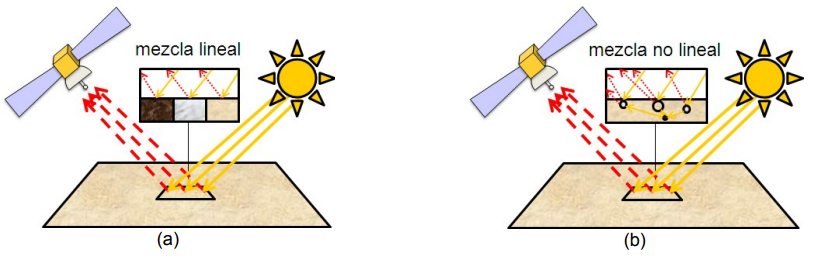
\includegraphics[width=\textwidth]{Imagenes/ComparativaModelosDesmezclado.png}
  \caption{Comparativa entre modelos de desmezclado espectral.}
  \label{fig:comparativa modelos de desmezclado espectral}
\end{figure}

La otra aproximación es el modelo no lineal de mezcla, que tiene en cuenta también aquellos endmembers que se distribuyen al azar a lo largo del campo de visión del sensor, por lo que proporciona una mejor información de la imagen. Sin embargo, para ello requiere información previa acerca de las propiedades físicas de los materiales que conforman la imagen. La Figura~\ref{fig:comparativa modelos de desmezclado espectral} \cite{biblio:TFG_Esquembri} se presenta una comparativa de los dos posibles modelos de desmezclado espectral. Como el modelo no lineal no es aplicable a zonas sobre las que no se posee ninguna información, en este trabajo se opta por utilizar el modelo lineal de mezcla.


Como se puede observar en la Figura~\ref{fig:representacion grafica del modelo lineal de mezcla} \cite{biblio:TFM_Pablo_VCA}, el modelo lineal se puede interpretar gráficamente mediante un espacio bidimensional, utilizando un diagrama de dispersión entre dos bandas de la imagen poco relacionadas entre sí. Todos los puntos de la imagen quedan englobados dentro del área formada por los puntos más extremos, es decir, los elementos espectralmente más puros, que serán los mejores candidatos para ser seleccionados como endmembers.

\begin{figure}
  \centering
    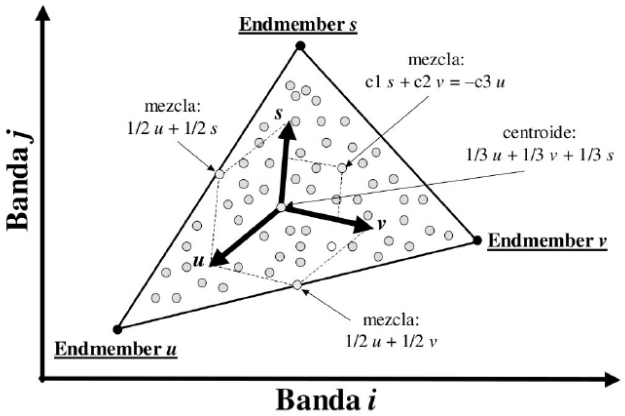
\includegraphics[width=0.7\textwidth]{Imagenes/GraficoModeloLinealDeMezcla.png}
  \caption{Representación gráfica del modelo lineal de mezcla.}
  \label{fig:representacion grafica del modelo lineal de mezcla}
\end{figure}

De esta manera se forman sistemas de coordenadas con origen en el centroide de la nube de puntos y los vectores que van de ese punto a los endmembers. Así, cualquier punto de la imagen puede expresarse como combinación lineal de los endmembers entre los que se encuentre. El paso clave a la hora de aplicar el modelo lineal de mezcla consiste, pues, en identificar de forma correcta los elementos extremos de la nube de puntos N-dimensional. Para ello existen numerosos algoritmos de extracción de endmembers, como el Automatic Target Detection and Classification Algorthm empleado en el presente trabajo.

Se ha optado por el algoritmo ATDCA-GS ya que en trabajos previos se ha hecho uso de arquitecturas CPUs o GPUs y el rendimiento obtenido ha sido suficiente para poder realizar un procesamiento en tiempo real, además de que puede mejorar la precisión si se compara con el algoritmo ATDCA-OSP. También se trata de un algoritmo sencillo pero al mismo tiempo bastante robusto, con operaciones no muy costosas en términos computacionales. Por ejemplo, si de nuevo lo comparamos con el algoritmo ATDCA-OSP, la operación de calcular la inversa de una matriz para obtener las proyecciones ortogonales se sustituyen por la optimización del método de Gram Schmidt, de manera que la complejidad y el tiempo de ejecución se reducen considerablemente.

\section{Necesidad de paralelización}

La mayoría de las técnicas de análisis hiperespectral desarrolladas hasta la fecha, incluyendo la utilizada en este trabajo, tienen en cuenta que gran parte de los píxeles obtenidos por el sensor (píxeles mezcla) vienen dados por la contribución de diversos materiales que residen a nivel de sub-píxel. Por ello, son necesarios diseños capaces de modelar este fenómeno de manera adecuada, lo cual supone un coste computacional considerablemente alto.

Además, la elevada cantidad de datos que se obtienen de cada imagen hiperespectral (las bandas puede ser de cientos o incluso miles de longitudes de onda diferentes) no sólo dificulta la manera en que estos deben ser almacenados y procesados en un ordenador determinado, sino que añade la complicación de que esta información debe ser enviada previamente por el satélite que se ha encargado de la toma de las imágenes.

Existen posibles soluciones al problema de la alta dimensionalidad de los datos \cite{biblio:reducir_dimensiones}. Por un lado, se podría realizar una compresión de datos con pérdidas (mayor compresión pero menos información) o sin pérdidas (menor compresión pero manteniendo la información) \cite{biblio:compresion}. Por otro lado, se podría recoger de manera selectiva determinadas bandas espectrales en base a los materiales sobre los que se requiera información, por ejemplo, minerales y rocas en zonas mineras; o vegetación y agua en zonas de selva o bosque.

Debido a lo anterior, unido a que muchas aplicaciones de observación remota requieren capacidades de procesamiento en tiempo real, se hace imprescindible el uso de arquitecturas paralelas para el procesamiento eficiente y rápido de este tipo de imágenes. Esta tarea resulta relativamente sencilla puesto que al analizar las imágenes se hace uso de operaciones matriciales cuyo carácter repetitivo las hace altamente susceptibles de ser implementadas en arquitecturas paralelas.

En la actualidad, existen múltiples alternativas hardware para la computación paralela: procesadores multi-cores, GPUs o hardware dedicado como los Circuitos Integrados de Aplicación Específica (ASICs) o las FPGAs. De todas ellas, estas últimas presentan una opción eficiente en cuanto a rendimiento haciendo que los tiempos de respuesta sean reducidos y que el algoritmo se ejecute de manera más eficiente. También utiliza una cantidad menor de recursos, por lo que es una de las pocas alternativas que se pueden adaptar en un sensor para poder realizar un procesamiento a bordo.